\section{Interest Flooding in NDN}
\label{sec:interest flooding}

% Points here:
% - Definition of the Interest flooding attack
% - What makes Interest attack effective
% - Assumptions about the network, attackers, attack traffic, and legitimate consumers
% - References about other attacks and explicitly stating that this work aims to build a baseline for general Interest Flooding mitigation problem, with other attack profiles and malicious gateways.

NDN uses a pull-based data retrieval model which means that the network is always open for accepting incoming Interest packets in order to return Data back since NDN does not have any form of client authentication.

Interest flooding attack can be performed by a large set (possibly geographically distributed) of malicious clients (bots) that are injecting Interest packets into the network at a very fast pace. Interest flooding attack has devastating effects for the following reasons. 

Pending Interest Table (PIT) is used to keep per packet forwarding state in NDN and is critical for Data delivery. Though PIT table has an upper limit on its size, it doesn't prevent attacker from injecting a huge number of false Interest packets at a very high rate, which eventually will lead to a situation where the whole PIT table is full of false Interest packets and is not able to keep forwarding state of Interests coming from legitimate users. In this view it may look similar to TCP SYN-flood attack.

Another huge negative effect of Interest flooding attack is bandwidth exhaustion. In case if Interest flooding attack is performed using existing or static name prefixes, Content Store (CS) effectively prevents bandwidth exhaustion by caching static content along the route and bringing this static Data closer to attacking bots. However, if Interest flooding attack is performed using name prefixes for dynamically generated or non-existing content, Content Store can do nothing against this and bandwidth upstream to the content producer will be exhausted.

Interest Flooding attack that uses name prefixes for dynamically generated content belongs to application layer attacks and requires knowing application specific semantics. In this paper we are considering network level attacks performed by sending Interests with for non-existing data using prefix names with some random components. We make the assumption that the set of malicious clients (botnet) has a greedy behavior and tries to send as many false Interest packets as possible at any time given its connectivity options. Though NDN is capable of multipath Interest forwarding and forwarding strategy switching, we are using Best Route (single path) forwarding strategy in all of our experiments. 

This work aims to build a baseline for general Interest Flooding mitigation problem, with other attack profiles (smart and non-greedy) and malicious gateways (NDN routers inside the network perimeter) being left for a future work. Also we want to mention other possible DoS attacks in NDN architecture, such as 


%Any DoS attack aims to exhaust system resources. In the context of NDN by term "system" we understand two things: 1) each individual NDN router 2) a distributed system consisting of some collection of NDN routers. In a first case, every major data structure (FIB, CS, PIT) is a potential surface for denial of service attack. In a second case, we consider: 1) bandwidth between NDN routers 2) caching capabilities of NDN routers 3) packet processing capabilities of NDN routers.

%Let's examine an individual NDN router first. Certainly, as any other piece of software each specific NDN implementation can have bugs and exploits e.g. buffer overflows leading to data corruption in cache, etc. In this paper we are assuming an idealized NDN implementation lacking any implementation bugs. 

%In a general case, Forwarding Interest Base (FIB) is managed by routing protocol and if attackers have been able to get control over routing, they could advertise a huge number of FIB announcements that will fill up FIB table that may cause Interest processing delays and traffic redirection with amplification or black-holing.

%Pending Interest Table (PIT) is used to keep per packet forwarding state in NDN and is critical for Data delivery. Though PIT table has an upper limit on its size, it doesn't prevent attacker from injecting a huge number of false Interest packets at a very high rate, which eventually will lead to a situation where the whole PIT table is full of false Interest packets and is not able to keep forwarding state of Interests coming from legitimate users. This attack may look similar to TCP SYN-flood attack and we call it Interest flooding. 

%Content Store (CS) is an effective obstacle for several types of DDoS attacks. CS possesses two important characteristics: maximum size and replacement policy. However, by knowing replacement policy attacker can construct a specific traffic generator that is using weaknesses of a chosen replacement procedure that will lead to increased processing time, slower packet delivery and in some cases de facto a complete inability to cache legitimate data. 

%The primary goal behind any flooding denial of service attack is to overwhelm network, CPU, or memory resources on routers or the target host.


% An infrastructure consisting of NDN routers is vulnerable to the following types of attacks: 
% \begin{enumerate}
% \item Interest flooding. 
% \item fkjgkfjgkfg
% \end{enumerate} 


%\begin{figure}[htpb]
%  \centering
%  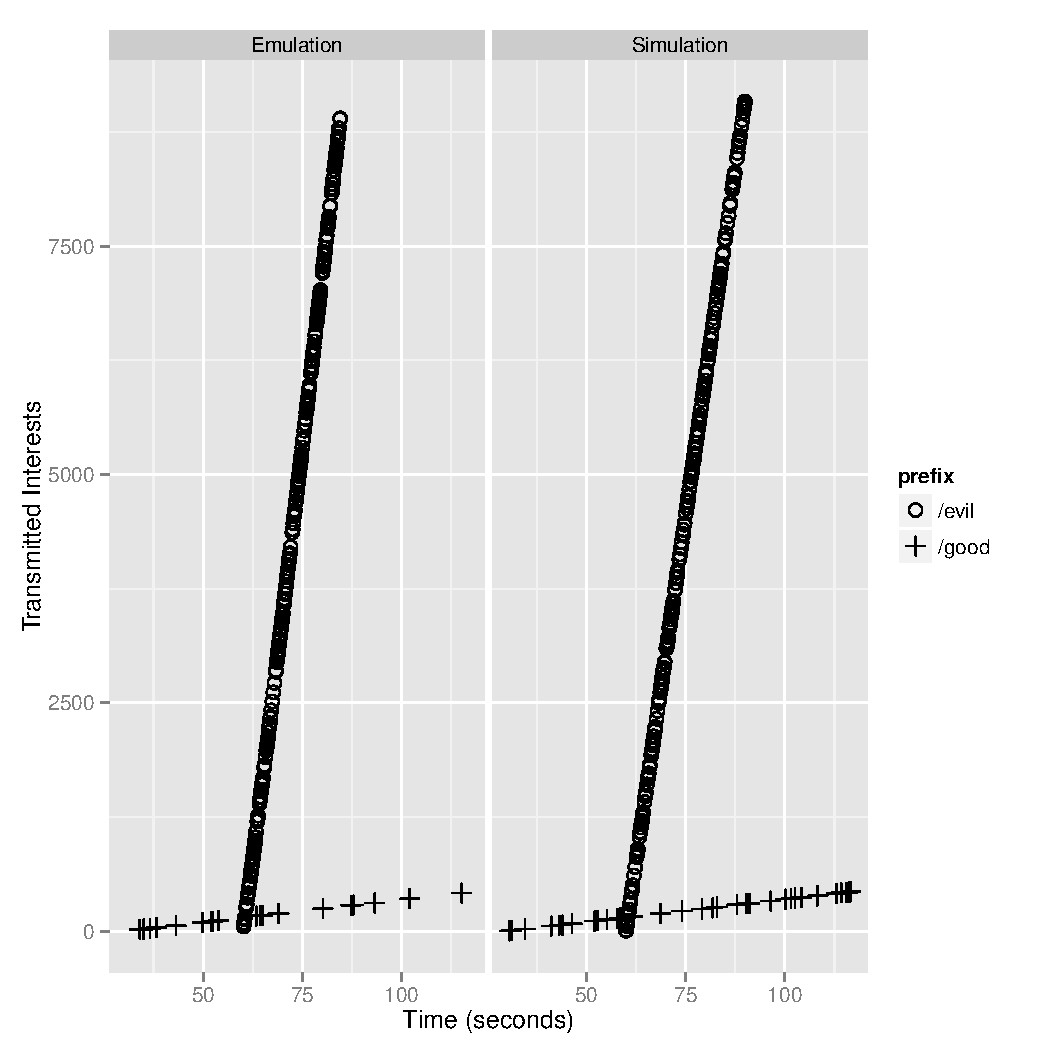
\includegraphics[scale=0.5]{figures/sim-emu-power.pdf}
%  \caption{Strength of Interest flooding attack}
%  \label{fig:simemupower}
%\end{figure}

%\begin{figure}[htpb]
%  \centering
%  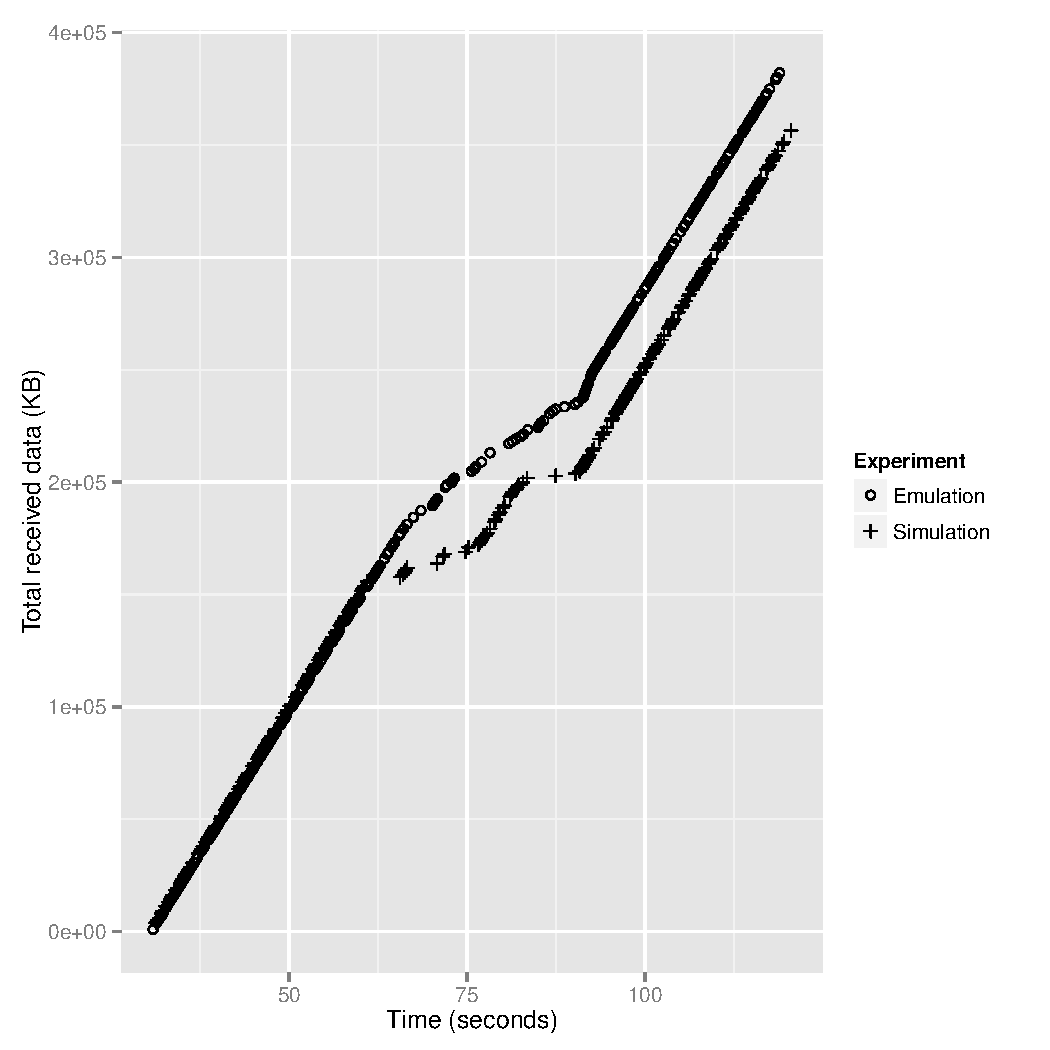
\includegraphics[scale=0.5]{figures/sim-emu-performance.pdf}
%  \caption{Data retrieval by legitimate clients}
%  \label{fig:simemuperf}
%\end{figure}


%%% Local Variables: 
%%% mode: latex
%%% TeX-master: "paper"
%%% End: 
